\documentclass[fontset=windows,a4paper,12pt]{ctexart}
\usepackage{geometry}
\usepackage{graphicx}
\usepackage{subfigure}
\usepackage{graphics}
%\usepackage{overcite}
\usepackage{listings}
\usepackage{CJK}

\pagestyle{plain}
\usepackage{bm}
\usepackage{amsmath}
\usepackage{multirow}

\geometry{top=25mm,bottom=20mm,left=25mm,right=25mm}
\newcommand{\upcite}[1]{\textsuperscript{\textsuperscript{\cite{#1}}}}
\renewcommand{\eqref}[1]{公式 (\ref{#1})}
\renewcommand*{\baselinestretch}{1.38}

\begin{document}
  \begin{center}
  	\zihao{3}{\heiti 小区开放对道路通行的影响}
  \end{center}
  \linespread{1.2}
  \begin{center}
  	\zihao{4}{\heiti 摘\ \ \ \ 要}
  \end{center}
  \zihao{4}{\songti 
  	
  	摘要摘要摘要摘要
  	摘要摘要摘要摘要
  	摘要摘要摘要摘要
  	摘要摘要摘要摘要
  	摘要摘要摘要摘要

  }
  \textbf{关键词:}\ 层次分析\ 元胞自动机
  
  \section{问题重述}
  \section{符号说明}
  \section{问题分析}
	\subsection{问题一}
		\subsubsection{Braess悖论}
			数学家Dietrich Braess在1968年首次提出了Braess悖论\upcite{Braess1968Ü}。
			考虑拓扑结构如图\ref{fig:braess}的交通网,假设交通网中的流量为4000,起点为A,终点为D
			通过$ A \rightarrow B $与$ C \rightarrow D $的时间均为车流量除以100,通
			过$ B \rightarrow D $与$ A \rightarrow C $的时间为固定的45分钟。
			\begin{figure}[!htbp]
				\centering
				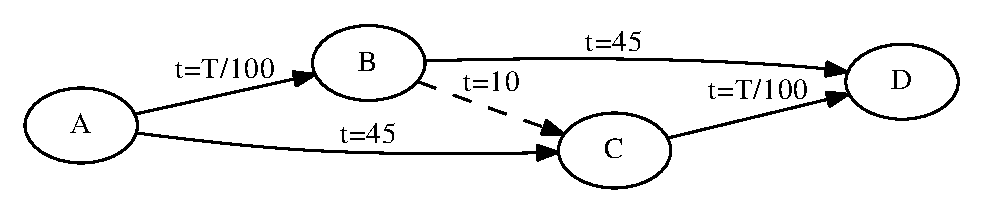
\includegraphics[width=0.5\textwidth]{pic/braess.eps}
				\caption{Braess悖论的具体情况}
				\label{fig:braess}
			\end{figure}
			在路径$ B \rightarrow C $没有开通时,从$ A \rightarrow D $的通过时间分别为$ \frac{A}{100}+45 $与$ \frac{B}
			{100} + 45 $,达到均衡之后有$ A=B=2000 $这样每条路通过的时间都是$ \frac{2000}{100}
			+45=65 $分钟。
			
			现在考虑$ B \rightarrow C $开通之后,其通过时间非常短,在这种情况下,所有司机都会选择$ A \rightarrow B \rightarrow C \rightarrow D $这条路线,因为即使所有车辆全部通过$ A \rightarrow B $所用时间也不超过40分钟,这样所有通过这条路径的时间为$ \frac{4000}{100}\times 2+10=90$分钟,Braess便是指这种情况。
	\subsection{问题二}
	考虑小区开放对周边道路通行的两个影响因素:道路条件、交通条件。
		\subsubsection{道路条件}
			首先,对小区周边道路条件进行分析。道路通行主要考虑从一点到另一点的实际通行时间,实际通行时间$ T=d_1+D $,其中$ d_1 $为延误时间,$ D $为行程时间。

			延误时间\upcite{任福田2003交通工程学}是指,道路上通行所需时间除行走时间外,也受市政道路交通信号灯的影响,如\eqref{eq:delay_func}所示。
			\begin{equation}
				d_1=\frac{0.5T(1-\frac{t_g}{T})}{1-[min(1,x)\cdot{\frac{t_g}{T}}]}
				\label{eq:delay_func}
			\end{equation}
			其中$ T $表示信号灯周期长度,$ t_g $代表绿灯时间,$ x $代表最大交通量与基本交通量之比。
			
			通行时间是指,在不考虑交通路口的通行状况下,通过某个路段所需时间。常用的通行时间函数
			美国联邦公路局函数(即BPR函数)如\eqref{bpr_plain}所示。
			\begin{equation}
				t_{ij}=\alpha_{ij}+\beta_{ij}f_{ij}
				\label{bpr_plain}
			\end{equation}
			其中$ ij $表示从i路段到j路段,$ t_{ij} $表示在该路段所花的时间,$ \alpha_{ij} $为路段上的
			结合具体情况,对其改进\upcite{李向朋2014城市交通拥堵对策—封闭型小区交通开放研究}
			,考虑到小区内道路上行人、自行车等非机动车较多的
			特点,增加行人对机动车的影响、自行车对机动车的影响。结合已有的研究成果,得到行人
			、自行车分别对车辆的影响系数,得到改进BPR函数。BPR阻抗函数为:
					
		\subsubsection{行程时间}
		\subsubsection{车流量}
			
	\subsection{问题二}
		综合问题一的评价模型建立元胞自动机模型
		\begin{equation}
			A=(L,d,S,N,f)
		\end{equation}
		其中A代表自动机模型,其中L为元胞空间;d为元胞空间的维数;S为状态集合;N为某个邻域内所有元胞的集合;f为局部映射或局部规则。
		根据问题一中的模型,建立一个二维元胞自动机模型,每个每个元胞具有几个固定的生成地点,在
		$ L $中有确定的目的地。
  \newpage
  \bibliography{mybib}
  \bibliographystyle{gbt7714}

\end{document}